\documentclass[12pt]{article}


\newcommand{\hmwkTitle}{Homework \# 3}
\newcommand{\hmwkDueDate}{\today}
\newcommand{\hmwkClass}{PHSX 611}
\newcommand{\hmwkAuthorName}{\textbf{Grant Saggars}}



\usepackage{fancyhdr}
\setlength{\headheight}{15pt}
\usepackage{extramarks}
\usepackage{amsmath}
\usepackage{amsthm}
\usepackage{amsfonts}
\usepackage{tikz}
\usepackage{pgfplots}
\usetikzlibrary{calc}

\usepackage{float}
\usepackage{caption}
\usepackage{bbold}
\usepackage{xcolor}
\usepackage{framed}
\usepackage{enumerate}
\usepackage{cancel}
\usepackage{multicol}
\usepackage{XCharter}

\usetikzlibrary{automata,positioning}

\usepackage{geometry}
\geometry{top=1in, bottom=1in, left=1in, right=1in} % Adjust margins as needed

\pagestyle{fancy}
\lhead{\hmwkAuthorName}
\chead{\hmwkClass\: \hmwkTitle}
\rhead{\firstxmark}
\lfoot{\lastxmark}
\cfoot{\thepage}

%
% Basic Document Settings
%

\topmargin=-0.75in
\evensidemargin=0in
\oddsidemargin=0in
\textwidth=6.5in
\textheight=9.0in
\headsep=0.25in

\linespread{1.1}

\renewcommand\headrulewidth{0.4pt}
\renewcommand\footrulewidth{0.4pt}

\setlength\parindent{0pt}

%
% Create Problem Sections
%

\newcommand{\enterProblemHeader}[1]{
    \nobreak\extramarks{}{Problem \arabic{#1} continued on next page\ldots}\nobreak{}
    \nobreak\extramarks{Problem \arabic{#1} (continued)}{Problem \arabic{#1} continued on next page\ldots}\nobreak{}
}

\newcommand{\exitProblemHeader}[1]{
    \nobreak\extramarks{Problem \arabic{#1} (continued)}{Problem \arabic{#1} continued on next page\ldots}\nobreak{}
    \stepcounter{#1}
    \nobreak\extramarks{Problem \arabic{#1}}{}\nobreak{}
}

\setcounter{secnumdepth}{0}
\newcounter{partCounter}
\newcounter{homeworkProblemCounter}
\setcounter{homeworkProblemCounter}{1}
\nobreak\extramarks{Problem \arabic{homeworkProblemCounter}}{}\nobreak{}

%
% Homework Problem Environment
%
% This environment takes an optional argument. When given, it will adjust the
% problem counter. This is useful for when the problems given for your
% assignment aren't sequential. See the last 3 problems of this template for an
% example.
%
\newenvironment{homeworkProblem}[1][-1]{
    \ifnum#1>0
        \setcounter{homeworkProblemCounter}{#1}
    \fi
    \section{Problem \arabic{homeworkProblemCounter}}
    \setcounter{partCounter}{1}
    \enterProblemHeader{homeworkProblemCounter}
}{
    \exitProblemHeader{homeworkProblemCounter}
}

%
% Callout Box
%

\definecolor{shadecolor}{RGB}{235,235,235}
\newenvironment{callout}[1] {\begin{shaded*} \textbf{#1}} {\end{shaded*}}

%
% Title Page
%

\title{
    \textmd{\textbf{\hmwkClass:\ \hmwkTitle}}\\
    \normalsize\vspace{0.1in}\small{\hmwkDueDate}\\
}

\author{\hmwkAuthorName}
\date{}

\renewcommand{\part}[1]{\textbf{\large Part \Alph{partCounter}}\stepcounter{partCounter}\\}





\begin{document}

\maketitle

\begin{homeworkProblem}
	We learned in Section 2.3 what a commutator of operators $[\hat{A}, \hat{B}]$ is. Derive commutators of the following:
	\begin{enumerate}[a)]
		\item Potential energy $V(x)$ and momentum operator $\hat{p}$;
		      \begin{callout}{Solution:}
			      \begin{align*}
				      \widehat{V} & = V(x)                                  \\
				      \hat{p}     & = -i \hbar \frac{\partial }{\partial x} \\
			      \end{align*}
			      \begin{align*}
				      [\widehat{V},\hat{p}]f          & = \widehat{V}\hat{p} - \hat{p}\widehat{V}                                          \\
				                                      & = V(x) (-i \hbar) \frac{d}{dx}(f) - (-i \hbar) \frac{d}{dx}(V(x)f)                 \\
				                                      & = -i \hbar \left( \frac{df}{dx}V(x) - \frac{df}{dx}V(x) - \frac{dV(x)}{dx}f\right) \\
				                                      & = i \hbar f \frac{dV(x)}{dx}                                                       \\
				      \implies [\widehat{V}, \hat{p}] & = i \hbar \frac{dV}{dx}
			      \end{align*}
		      \end{callout}
		      \newpage \item Kinetic energy operator $\widehat{T}$ and momentum operator $\hat{p}$;
		      \begin{callout}{Solution:}
			      \begin{align*}
				      \widehat{T} & = \frac{\hat{p}^{2}}{2m}                \\
				      \hat{p}     & = -i \hbar \frac{\partial }{\partial x} \\
			      \end{align*}
			      \begin{align*}
				      [\widehat{T}, \hat{p}] & = \widehat{T}\hat{p} - \hat{p}\widehat{T}                      \\
				                             & = \left( \frac{\hat{p}^{2}}{2m} \right) \left( \hat{p} \right)
				      - \left( \hat{p} \right) \left( \frac{\hat{p}^{2}}{2m} \right)                          \\
				                             & = \frac{1}{2m} \left( \hat{p}^2 \left( \hat{p} \right)
				      - \left( \hat{p} \right) \hat{p}^2  \right)                                             \\
				                             & = \frac{1}{2m} \left( \hat{p}[\hat{p}, \hat{p}]
				      - [\hat{p}, \hat{p}]\hat{p} \right)
			      \end{align*}

			      Because operators commute with themselves, $[\hat{p}, \hat{p}]$ equals zero.

			      \begin{align*}
				      [\widehat{T}, \hat{p}] & = 0
			      \end{align*}

		      \end{callout}
		\item Hamiltonian operator $\widehat{H}$ and momentum operator $\hat{p}$;
		      \begin{callout}{Solution:}

			      \begin{align*}
				      \widehat{H} & = \widehat{T} + \widehat{V} = \frac{\hat{p}^{2}}{2m} + V(x) \\
				      \hat{p}     & = -i \hbar \frac{\partial }{\partial x}
			      \end{align*}
			      \begin{align*}
				      [\widehat{H},\hat{p}] & = [\widehat{T}+\widehat{V}, \hat{p}] = \cancelto{0}{[\widehat{T}, \hat{p}]} + \cancelto{ih \frac{dV}{dx}}{[\widehat{V}, \hat{p}]} \\
				                            & = i \hbar \frac{dV}{dx}
			      \end{align*}

		      \end{callout}
		      \newpage \item Define the condition at which $[\widehat{H}, \hat{p}]=0$. (0.25 pt.)
		      \begin{callout}{Solution:}
			      If $V(x)$ is constant or independent of position, $\frac{dV}{dx}$ goes to zero, making the operator commute.
		      \end{callout}
	\end{enumerate}
\end{homeworkProblem}

\begin{homeworkProblem}
	Calculate the commutator of raising and lowering operators: $\left[\widehat{a_{+}}, \widehat{a_{-}}\right] .(0.25 \mathrm{pt}$.)

	\begin{callout}{Solution:}
		$$ a_{\pm} = \frac{1}{\sqrt{ 2m \hbar \omega }} \left( \mp i \hat{p} + m \omega \hat{x} \right) $$

		\begin{align*}
			\left[\widehat{a_{+}}, \widehat{a_{-}}\right] & =
			\frac{1}{2m \hbar \omega } \left( - i \hat{p} + m \omega \hat{x} \right) \left( i \hat{p} + m \omega \hat{x} \right)
			- \frac{1}{2m \hbar \omega } \left( i \hat{p} + m \omega \hat{x} \right) \left( - i \hat{p} + m \omega \hat{x} \right) \\
			                                              & = 0
		\end{align*}
	\end{callout}

\end{homeworkProblem}

\begin{homeworkProblem}
	(Problem 2.7) Infinite square well. A particle in the infinite square well has the initial wave function:
	$$
		\Psi(x, 0)=\left\{\begin{array}{c}
			A x, 0 \leq x \leq a / 2 \\
			A(a-x), a / 2 \leq x \leq a
		\end{array}\right.
	$$
	\begin{enumerate}[a)]
		\item Sketch $\Psi(x, 0)$, and determine the constant $A$ (normalize wavefunction).

		      \begin{callout}{Solution:}

			      \begin{align*}
				      1   & = \int_{0}^{a/2} A ^{2} x ^{2} ~dx + \int_{a/2}^{a} A ^{2}(a-x)^{2} ~dx \\
				      1   & = \frac{A^2a^3}{24} + \frac{A^2a^3}{24} \to \frac{2A^2a^3}{24}          \\
				      A^2 & = \frac{24}{2a^3}                                                       \\
				      A   & = \sqrt{ \frac{12}{a^3} }
			      \end{align*}

			      \vspace{0.3cm}
			      A plot of the above wavefunction is:

			      \center 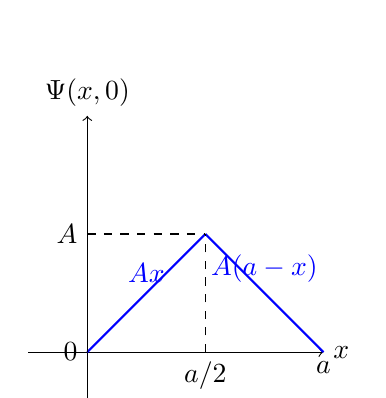
\begin{tikzpicture}[scale=1.5]
				      % Axes
				      \draw[->] (-0.5,0) -- (2,0) node[right] {$x$};
				      \draw[->] (0,-0.5) -- (0,2) node[above] {$\Psi(x,0)$};
				      % Function
				      \draw[blue, thick] (0,0) -- (1,1) node[midway, above] {$A x$};
				      \draw[blue, thick] (1,1) -- (2,0) node[midway, above] {$A(a-x)$};
				      % Points and labels
				      \draw[dashed] (1,0) node[below] {$a/2$} -- (1,1);
				      \draw[dashed] (0,1) node[left] {$A$} -- (1,1);
				      \draw[dashed] (0,0) node[left] {$0$} -- (0,1);
				      \draw[dashed] (2,0) node[below] {$a$} -- (2,0);
			      \end{tikzpicture}

		      \end{callout}
		\item Find $\Psi(x, t)$.
		      \begin{callout}{Solution:}

			      Begin by finding $c_n$:
			      \begin{align*}
				      c_n & = \int \psi_n^* \Psi(x,0) ~dx                                                                                                                                               \\
				          & = \left\{\begin{array}{ll}
					                     \frac{2}{a} \int_0^{a/2} \sqrt{ \frac{12}{a^3} } x \sin\left( \frac{n\pi x}{a} \right)~dx,       & 0 \leq x \leq a/2 \\
					                     \frac{2}{a} \int_{a/2}^{a} \sqrt{ \frac{12}{a^3} } (a-x) \sin\left( \frac{n\pi x}{a} \right)~dx, & a/2 \leq x \leq a
				                     \end{array}\right.                                       \\
				          & = \left\{\begin{array}{ll}
					                     \frac{2\sqrt{3}\left(2\sin \left(\frac{\pi n}{2}\right)-\pi n\cos \left(\frac{\pi n}{2}\right)\right)}{\pi ^2n^2\sqrt{a}}, & 0 \leq x \leq a/2 \\
					                     \frac{2\sqrt{3}\left(\pi n\cos \left(\frac{\pi n}{2}\right)+2\sin \left(\frac{\pi n}{2}\right)\right)}{\pi ^2n^2\sqrt{a}}, & a/2 \leq x \leq a
				                     \end{array}\right.
			      \end{align*}

			      The general solution is therefore (leaving the $c_n$'s symbolic to save space on the page):

			      \begin{align*}
				      \Psi(x,t) & = \left\{
				      \begin{array}{ll}
					      \sqrt{ \frac{12}{a^3} } \sum c_n x \exp\left( \frac{-i E_n}{\hbar}t \right),     & 0 \leq x \leq a/2 \\
					      \sqrt{ \frac{12}{a^3} } \sum c_n (a-x) \exp\left( \frac{-i E_n}{\hbar}t \right), & a/2 \leq x \leq a \\
				      \end{array} \right.
			      \end{align*}

		      \end{callout}
		      \newpage \item What is the probability that a measurement of the energy would yield the value $E_1$.
		      \begin{callout}{Solution:}

			      The expectation value for energy is defined as $\sum c_n^2 E_n$, where the square of $c_n$ goes to 1 at infinity; consequently, $c_n^2$ is the probability to measure a given energy, so:

			      \begin{align*}
				      P(E_1) & = c_{n1}c_{n1}^{*}                                                                                                                                                               \\
				             & = \left\{ \begin{array}{ll}
					                         \frac{12\left(2\sin \left(\frac{\pi (1)}{2}\right)-\pi (1)\cos \left(\frac{\pi (1)}{2}\right)\right)^2}{\pi ^4(1)^4a}, & 0 \leq x \leq a/2 \\
					                         \frac{12\left(\pi (1)\cos \left(\frac{\pi (1)}{2}\right)+2\sin \left(\frac{\pi (1)}{2}\right)\right)^2}{\pi ^4(1)^4a}, & a/2 \leq x \leq a
				                         \end{array} \right.
			      \end{align*}

			      This of course depends on the barrier width, $a$.

		      \end{callout}
		\item Find the expectation value of the energy (it doesn't matter how you will achieve that). (0.5 pt.)
		      \begin{callout}{Solution:}

			      Using the expectation value for the Hamiltonian defined in terms of $\hat{T}, \hat{V}$:

			      (I believe this only involves the time-independent equation, not the generalized form)

			      \begin{align*}
				      \langle \hat{H} \rangle & = \int_{0}^{a/2} \psi^*_{I} \hat{H} \psi_{I} ~dx
				      + \int_{a/2}^{a} \psi^*_{II} \hat{H} \psi_{II} ~dx                                                                                                                               \\
				                              & = \int_{0}^{a/2} - \frac{\hbar ^{2}}{2m} \cancelto{\frac{24}{a^3}}{\frac{\partial ^{2}}{\partial x ^{2}} \frac{12}{a^3}x^2} + \frac{12}{a^3}(x)^2V ~dx
				      + \int_{a/2}^{a} - \frac{\hbar ^{2}}{2m} \cancelto{\frac{24}{a^3}}{\frac{\partial ^{2}}{\partial x ^{2}}\frac{12}{a^3}(a-x)^2} + \frac{12}{a^3}(a-x)^2V ~dx                      \\
				                              & = \int_{0}^{a/2} -\frac{\hbar ^{2}}{2m} \frac{24}{a^3} + \frac{12}{a^3}x^2V ~dx
				      + \int_{a/2}^{a} \frac{-\hbar ^{2}}{2m} \frac{24}{a^3} + \frac{12}{a^3}(a-x)V ~dx                                                                                                \\
				                              & = \frac{\hbar ^{2}}{2m} \left( \frac{24}{a^2} \right) + V
			      \end{align*}

		      \end{callout}
	\end{enumerate}
\end{homeworkProblem}

\newpage
\begin{homeworkProblem}
	(Problem 2.10) Harmonic oscillator.
	\begin{enumerate}[a)]
		\item Construct $\psi_2(x)$.
		      \begin{callout}{Solution:}
			      $$ \psi_n = A_n \hat{a}_{+}^{n}\psi_0 $$
			      $$ \psi_0 = \left( \frac{m\omega}{\pi \hbar} \right)^{1/4}\exp\left( -\frac{m\omega}{2\hbar}x^{2} \right) $$

			      \begin{align*}
				      \psi_1 & = A_1\hat{a}_{+}\psi_0 = \frac{A_1}{\sqrt{ 2 \hbar m \omega}} \left( -\hbar \frac{d}{dx}+m\omega x \right)\left( \frac{m\omega}{\pi \hbar} \right)^{1/4} e^{-\frac{m\omega}{2 \hbar}x } \\
				             & = A_{1} \left( \frac{m\omega}{\pi \hbar} \right)^{1/4}\sqrt{ \frac{2m\omega}{\hbar}}xe^{-m\omega x^2/2\hbar}
			      \end{align*}

			      \begin{align*}
				      \psi_2 & = \frac{A_{1}}{\sqrt{ 2m\hbar\omega }}\left( -\hbar \frac{d}{dx} + m\omega x \right) \left( \frac{m\omega}{\pi \hbar} \right)^{1/4}\sqrt{ \frac{2m\omega}{\hbar}}xe^{-m\omega x^2/2\hbar}                                                         \\
				             & = \frac{A_{1}}{\sqrt{ 2m\hbar\omega }} \left( -\hbar\left( \frac{m\omega}{\pi \hbar} \right)^{1/4}\sqrt{ \frac{2m\omega}{\hbar} }\left( e^{-m\omega x^2/2\hbar} + \left( -\frac{m\omega}{\hbar} \right)x^2e^{-m\omega x^2/2\hbar} \right) \right) \\
				             & +(m\omega x)\left( \frac{m\omega}{\pi \hbar} \right)^{1/4}\sqrt{ \frac{2m\omega}{\hbar}}xe^{-m\omega x^2/2\hbar}                                                                                                                                  \\
				             & = A_{2} \left( \frac{m\omega}{\pi \hbar} \right)^{1/4}\left( \frac{2m\omega}{\hbar}x^{2}-1 \right) \exp\left( -\frac{m\omega}{2\hbar}x^{2} \right)
			      \end{align*}

		      \end{callout}

		      \newpage
		\item Sketch $\psi_0(x), \psi_1(x), \psi_2(x)$.
		      \begin{callout}{Solution:}

			      \begin{centering}
				      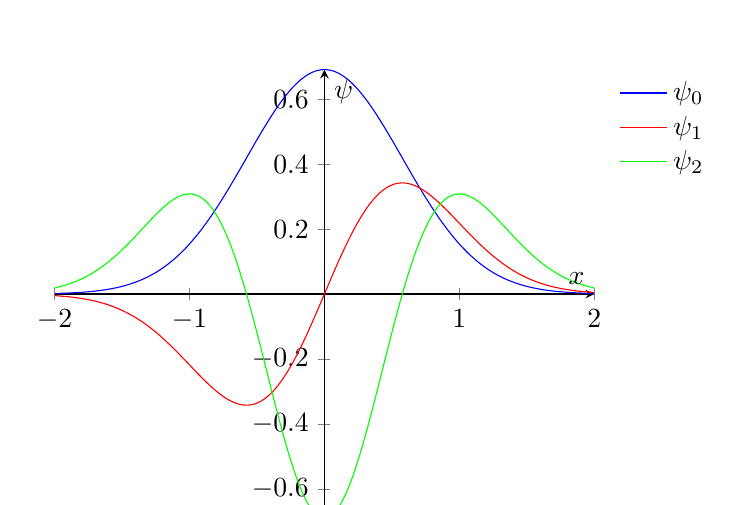
\begin{tikzpicture}
					      \begin{axis}[
							      xlabel=$x$,
							      ylabel=$\psi$,
							      domain=-2:2,
							      samples=100,
							      axis lines=middle,
							      legend pos=outer north east,
							      legend style={draw=none}
						      ]
						      % Define the functions
						      \def\psiZero{sqrt(1.5/pi) * exp(-1.5*x^2)}
						      \def\psiOne{x*sqrt(3/pi) * exp(-1.5*x^2)}
						      \def\psiTwo{(3*x^2-1)*sqrt(3/(2*pi)) * exp(-1.5*x^2)}
						      % Plot the functions
						      \addplot[blue,smooth] {\psiZero};
						      \addlegendentry{$\psi_0$}
						      \addplot[red,smooth] {\psiOne};
						      \addlegendentry{$\psi_1$}
						      \addplot[green,smooth] {\psiTwo};
						      \addlegendentry{$\psi_2$}
					      \end{axis}
				      \end{tikzpicture}

			      \end{centering}

		      \end{callout}
		\item Check the orthogonality of $\psi_0(x), \psi_1(x), \psi_2(x)$ by explicit integration. ( $0.5 \mathrm{pt}$.)
		      \begin{callout}{Solution:}

			      \begin{enumerate}[(1)]
				      \item $\psi_0(x)$:
				            \begin{align*}
					            \int_{-\infty}^{\infty} \psi_1^* \psi_0 ~dx & =
					            \int_{-\infty}^{\infty} \left( \frac{m\omega}{\pi \hbar} \right)^{1/4}\sqrt{ \frac{2m\omega}{\hbar}}xe^{-m\omega x^2/2\hbar}
					            \left( \frac{m\omega}{\pi \hbar} \right)^{1/4}\exp\left( -\frac{m\omega}{2\hbar}x^{2} \right) ~dx                \\
					                                                        & =
					            \int_{-\infty}^{\infty} \left(\frac{2m^2 \omega^2}{\pi h^2}\right)^{\frac{1}{2}}xe^{-\frac{m \omega x^2}{h}} ~dx \\
					                                                        & =
					            \left.-\frac{1}{\sqrt{ 2\pi }}e^{-\frac{\omega mx^2}{h}} \right|_{-\infty}^{\infty}                              \\
					                                                        & = 0
				            \end{align*}

				      \item $\psi_1(x)$:
				            Because there is no complex component in these, the integration is identical as with $\psi_0$ above.

				      \item $\psi_2(x)$:
				            \begin{align*}
					            \int_{-\infty}^{\infty} \psi_0^* \psi_2 ~dx & =
					            \int_{-\infty}^{\infty} \left( \frac{m\omega}{\pi \hbar} \right)^{1/4}\sqrt{ \frac{2m\omega}{\hbar}}xe^{-m\omega x^2/2\hbar}
					            \left( \frac{m\omega}{\pi \hbar} \right)^{1/4}\left( \frac{2m\omega}{\hbar}x^{2}-1 \right) \exp\left( -\frac{m\omega}{2\hbar}x^{2} \right) ~dx \\
					                                                        & =
					            \int_{-\infty}^{\infty} \left(\frac{2m^2 \omega^2}{\pi \hbar^2}\right)^{\frac{1}{2}}x\exp\left( -\frac{m \omega x^2}{\hbar} \right) ~dx        \\
					                                                        & =
					            \left. -\frac{1}{\sqrt{ 2\pi }} \exp\left(  -\frac{mwx^2}{h} \right) \right|_{-\infty}^{\infty}
					                                                        & = 0
				            \end{align*}

			      \end{enumerate}
		      \end{callout}
	\end{enumerate}
\end{homeworkProblem}
\begin{homeworkProblem}
	(Problem 2.13) A particle in the harmonic oscillator potential starts out in the state:

	$$\Psi(x, 0)=A\left[3 \psi_0(x)+4 \psi_1(x)\right].$$
	\begin{enumerate}[a)]
		\item Find $A$.
		      \begin{callout}{Solution:}

			      As a note to myself, here I attempted the normalization, moved on, then remembered the properties of orthonormal wave functions. The normalization can be greatly simplified by applying them:

			      \begin{align*}
				      1 & = \int_{-\infty}^{\infty} A^2[3\psi_0 + 4\psi_1][3\psi^*_0 + 4\psi^*_1] ~dx                                                                                           \\
				        & = A^2 \int_{-\infty}^{\infty} \cancelto{9}{9\psi_0\psi_{0}^*} + \cancelto{0}{12\psi_0\psi_1^*} + \cancelto{0}{12\psi_1\psi_0^*} + \cancelto{16}{16\psi_1\psi_1^*} ~dx \\
				      A & = \sqrt{ \frac{1}{25} } = \frac{1}{5}
			      \end{align*}

		      \end{callout}
		\item Construct $\Psi(x, t)$ and $|\Psi(x, t)|^2$.
		      \begin{callout}{Solution:}
			      \begin{align*}
				      \Psi(x,t) & = \frac{3}{5}\psi_0(x) + \frac{4}{5}\psi_1(x)                                                                                                                                                                                                                                          \\
				                & = \left[\begin{array}{c}
						                          \frac{3}{5} \left( \frac{m \omega}{\pi \hbar} \right)^{1/4} \exp\left( -\frac{m \omega }{2\hbar}x^2 \right) \exp\left( \frac{-iE_0t}{\hbar} \right) \\
						                          + \frac{4}{5} \left( \frac{4m ^{3} \omega ^{3} }{\pi \hbar ^{3}} \right)^{1/4} x \exp\left( -\frac{m \omega }{2\hbar}x^2 \right) \exp\left( \frac{-iE_1t}{\hbar} \right)
					                          \end{array}\right]           \\
				                & = \left[\begin{array}{c}
						                          \frac{3}{5} \left( \frac{m \omega}{\pi \hbar} \right)^{1/4} \exp\left( -\frac{m \omega }{2\hbar}x^2 \right) \exp\left( \frac{-i \omega}{2} t \right) \\
						                          + \frac{4}{5} \left( \frac{4m ^{3} \omega ^{3} }{\pi \hbar ^{3}} \right)^{1/4} x \exp\left( -\frac{m \omega }{2\hbar}x^2 \right) \exp\left( \frac{-3i \omega}{2} t \right) \tag{1}
					                          \end{array}\right]
			      \end{align*}

			      \newpage
			      \begin{gather*}
				      |\Psi(x,t)|^{2} = \Psi(x,t)\Psi^*(x,t) \\
				      = \left[\begin{array}{c}
						      \frac{3}{5} \left( \frac{m \omega}{\pi \hbar} \right)^{1/4} \exp\left( -\frac{m \omega }{2\hbar}x^2 \right) \exp\left( \frac{-i \omega}{2} t \right) \\
						      + \frac{4}{5} \left( \frac{4m ^{3} \omega ^{3} }{\pi \hbar ^{3}} \right)^{1/4} x \exp\left( -\frac{m \omega }{2\hbar}x^2 \right) \exp\left( \frac{-3i \omega}{2} t \right)
					      \end{array}\right] \\ \times
				      \left[\begin{array}{c}
						      \frac{3}{5} \left( \frac{m \omega}{\pi \hbar} \right)^{1/4} \exp\left( -\frac{m \omega }{2\hbar}x^2 \right) \exp\left( \frac{i \omega}{2} t \right) \\
						      + \frac{4}{5} \left( \frac{4m ^{3} \omega ^{3} }{\pi \hbar ^{3}} \right)^{1/4} x \exp\left( -\frac{m \omega }{2\hbar}x^2 \right) \exp\left( \frac{3i \omega}{2} t \right)
					      \end{array}\right]
			      \end{gather*}

			      Out of respect for myself, as I am writing this in \LaTeX, I will just skip to the simplified answer:

			      \begin{align*}
				      \frac{1}{25} \sqrt{ \frac{m \omega }{\pi \hbar} } \left[ 9 + \frac{32m \omega }{\hbar} x^{2} + 12 \sqrt{ \frac{2m \omega}{\hbar} }x \cancelto{\cos(\omega t)}{(e^{i \omega t} + e^{-i \omega t})}\right]\exp\left( - \frac{m \omega}{\hbar}x^2 \right) \tag{2}
			      \end{align*}
		      \end{callout}
		\item Find $\langle x\rangle$ and $\langle p\rangle$. (0.5 pt.)
	\end{enumerate}

	Note: you don't need to check if Ehrenfest's theorem holds as it is asked in Griffiths. We will come back to this theorem later in the course.

	\begin{callout}{Solution:}

		\begin{enumerate}[(1)]
			\item $\langle x \rangle$:
			      \begin{gather*}
				      \int_{-\infty}^{\infty}
				      x \frac{1}{25} \sqrt{ \frac{m \omega }{\pi \hbar} } \left[ 9 + \frac{32m \omega }{\hbar} x^{2} + 12 \sqrt{ \frac{2m \omega}{\hbar} }x \cos(\omega t)\right]\exp\left( - \frac{m \omega}{\hbar}x^2 \right) ~dx \\
				      = \frac{1}{25} \sqrt{ \frac{m \omega}{\pi \hbar} } \int_{-\infty}^{\infty} A+B+C ~dx
			      \end{gather*}
			      Let:
			      \begin{align*}
				      A & = 9x \exp\left( \frac{-m \omega}{\hbar}x^{2} \right)                                                   \\
				      B & = \frac{32 m \omega }{\hbar}x^3 \exp\left( \frac{-m \omega}{\hbar}x^{2} \right)                        \\
				      C & = 12 \sqrt{ \frac{2m \omega}{\hbar} }x^2\cos(\omega t) \exp\left( \frac{-m \omega}{\hbar}x^{2} \right)
			      \end{align*}

			      Integrating these separately gives:
			      \begin{align*}
				      A & = \left. \frac{9 \hbar}{m \omega} \exp\left( -\frac{m \omega}{\hbar}x^2 \right) \right|_{-\infty}^{\infty}
				      = 0                                                                                                            \\
				      B & = 0                                                                                                        \\
				      C & = \frac{1}{4} \sqrt{ \pi }
			      \end{align*}
			      $A_2$ threw me off and some research indicated $x$ to an odd power outside the exponent should make the integral go to zero due to "odd symmetry". Recombining these gives:
			      \begin{align*}
				      \frac{6}{25} \sqrt{ \frac{2 \hbar}{\pi m \omega} } \cos(\omega t)
			      \end{align*}

			\item $\langle p \rangle$:
			      \begin{align*}
				      \int_{-\infty}^{\infty} -i \hbar \frac{\partial }{\partial x} |\Psi|^2 ~dx
			      \end{align*}

			      (this is a terrible derivative and integral which makes me question my correctness, I should bring this up at office hours to inquire about an easier way to do this)

			      I'll make the substitution $\alpha = \frac{\sqrt{ \frac{2}{\pi} }m^2 \omega ^2 \cos(\omega t)}{\hbar^{2}} $, as this is a constant in the eyes of the integral.
			      I'll also substitute $\beta = \frac{m \omega \sqrt{\frac{m \omega}{h}} }{\sqrt{\pi} h}$.
			      Third, I'll substitute $\gamma = \frac{m \omega}{\hbar}$.

			      \begin{gather*}
				      i \hbar \int_{-\infty}^{\infty}
				      \frac{24}{25} \alpha x^2 e^{-\gamma x^2}
				      + \cancelto{0}{\frac{64}{25 \hbar} \beta x^3 e^{-\gamma x^2}}
				      % \cancel{+ \frac{64 m^2 x^3 \omega^2 \sqrt{\frac{m \omega}{h}} e^{-\frac{m x^2 \omega}{h}}}{25 \sqrt{\pi} h^2}}
				      -\frac{12 \hbar}{25} \alpha e^{-\gamma x^2}
				      - \cancelto{0}{\frac{46 \hbar}{25} \beta x e^{-\gamma x^2}} \\
				      = i \hbar\left(
				      \sqrt{ \frac{\pi}{4} } \frac{\alpha}{(\gamma)^{3/2}}
				      - \sqrt{ \pi } \frac{\alpha }{\gamma }
				      \right)
			      \end{gather*}

			      Making the substitutions gives:

			      $$
				      = i \hbar\left( \sqrt{ \frac{\pi}{4} } \frac{\sqrt{ \frac{2}{\pi} }m^2 \omega ^2 \cos(\omega t)}{\hbar^{2}(\frac{m \omega}{\hbar})^{3/2}} - \sqrt{ \pi } \frac{\sqrt{ \frac{2}{\pi} }m^2 \omega ^2 \cos(\omega t) }{\hbar^{2}\frac{m \omega}{\hbar} } \right)
			      $$


		\end{enumerate}
	\end{callout}

\end{homeworkProblem}
\end{document}
